\documentclass{article}
\usepackage[utf8]{inputenc}
\usepackage{geometry}
\usepackage{tikz}

\usepackage{graphicx}
\graphicspath{{images/}}

\usepackage{float}
\usepackage{caption}
\usepackage{subcaption}
\captionsetup{compatibility=false}

\usepackage{hyperref}
\hypersetup{
  colorlinks,
  citecolor=black,
  filecolor=black,
  linkcolor=black,
  urlcolor=blue
}

\title{Polytope}
\author{URL, Mathtician, }
\date{February 2021}

\begin{document}

\maketitle

\section{Introduction}
Welcome to the \href{https://discord.gg/invite/zMRu7T4}{Polytope Discord}!

\section{What is a polytope?}
Roughly speaking, a \textbf{polytope} is an $n$-dimensional shape.
As with many terms used on the Polytope Discord,
the word ``polytope'' can have a few definitions which are not completely equivalent.
All of the commonly-used ones, however, agree:
\begin{enumerate}
  \item
A polytope in $n$ dimensions (known hereafter as an $n$-polytope)
is made of \textbf{facets} which are $(n-1)$-polytopes.
\begin{itemize}
\item \textbf{Points} ($0$-polytopes) are the facets of \textbf{line segments} ($1$-polytopes),
\item which are the facets of \textbf{polygons} ($2$-polytopes),
\item which are the facets of \textbf{polyhedra} ($3$-polytopes),
\item which are the facets of \textbf{polychora} ($4$-polytopes), etc.
\end{itemize}
For the next criterion, consider the following figures ABC and DEF.
\end{enumerate}

\begin{center}
  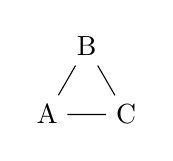
\begin{tikzpicture}
    \node (a) at (0,0) {A};
    \node (b) at (0.5,0.866) {B};
    \node (c) at (1,0) {C};
    \draw (a) -- (b) -- (c) -- (a);
  \end{tikzpicture}
  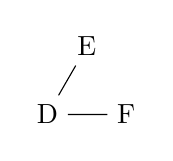
\begin{tikzpicture}
    \node (d) at (0,0) {D};
    \node (e) at (0.5,0.866) {E};
    \node (f) at (1,0) {F};
    \draw (e) -- (d) -- (f);
  \end{tikzpicture}
\end{center}

ABC is a triangle, a polygon with three line segments,
or \textbf{edges}, as they are known when mentioned as part of a larger polytope.
It also contains three points, or \textbf{vertices}, or even \textbf{verts} for short.
(In the polytope world, abbreviations are everywhere!)
DEF, on the other hand, is not a triangle; it is missing an edge,
leaving ``open ends'' at E and F which are each connected to only one edge.
To exclude DEF and figures like it,
we require that within a polygon, every vertex be connected to exactly two edges.
This condition also excludes ``branches'' where more than two edges meet at a vertex.

Let's generalize this rule to $n$-dimensional polytopes.
Two 3D figures are shown below.

\begin{center}
  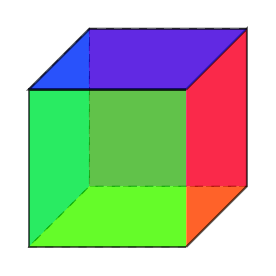
\begin{tikzpicture}
    \coordinate (A0) at (1,1,1);
    \coordinate (A1) at (1,1,-1);
    \coordinate (A2) at (1,-1,1);
    \coordinate (A3) at (1,-1,-1);
    \coordinate (A4) at (-1,1,1);
    \coordinate (A5) at (-1,1,-1);
    \coordinate (A6) at (-1,-1,1);
    \coordinate (A7) at (-1,-1,-1);
    \draw[dashed,fill=cyan,opacity=0.6] (A4) -- (A5) -- (A7) -- (A6);
    \draw[dashed,fill=magenta,opacity=0.6] (A1) -- (A5) -- (A7) -- (A3);
    \draw[dashed,fill=yellow,opacity=0.6] (A2) -- (A6) -- (A7) -- (A3);
    \draw[thick,fill=red,opacity=0.6] (A0) -- (A1) -- (A3) -- (A2);
    \draw[thick,fill=green,opacity=0.6] (A0) -- (A4) -- (A6) -- (A2);
    \draw[thick,fill=blue,opacity=0.6] (A0) -- (A4) -- (A5) -- (A1);
  \end{tikzpicture}  
  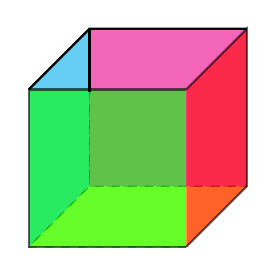
\begin{tikzpicture}
    \coordinate (A0) at (1,1,1);
    \coordinate (A1) at (1,1,-1);
    \coordinate (A2) at (1,-1,1);
    \coordinate (A3) at (1,-1,-1);
    \coordinate (A4) at (-1,1,1);
    \coordinate (A5) at (-1,1,-1);
    \coordinate (A6) at (-1,-1,1);
    \coordinate (A7) at (-1,-1,-1);
    \draw[dashed,fill=cyan,opacity=0.6] (A4) -- (A5) -- (A7) -- (A6);
    \draw[dashed,fill=magenta,opacity=0.6] (A1) -- (A5) -- (A7) -- (A3);
    \draw[dashed,fill=yellow,opacity=0.6] (A2) -- (A6) -- (A7) -- (A3);
    \draw[thick,fill=red,opacity=0.6] (A0) -- (A1) -- (A3) -- (A2);
    \draw[thick,fill=green,opacity=0.6] (A0) -- (A4) -- (A6) -- (A2);
    \draw[thick] (A4) -- (A5) -- (A1);
    \draw[thick] (A5) -- (-1,0.2,-1);
  \end{tikzpicture}  
\end{center}

The left figure is a cube, a polyhedron with
six square \textbf{faces}, twelve edges, and eight vertices.
The right is the same, but with the top face removed.
The right figure is not a polyhedron because, like DEF, it leaves ``open ends.''
However, in this case, the open ends are not vertices but the top four edges,
which are each connected to only one face.
We require that within a polyhedron, every edge be connected to exactly two faces.
\footnote{
  Our previous rule for polygons does not apply to the cube or to other polyhedra;
  every vertex of the cube is connected to three edges, not two.
  However, the rule does apply to each of the cube's faces.
}



Are you beginning to see a pattern?
In an $n$-polytope, removing an $(n-1)$-dimensional facet
creates ``open ends'' in the $(n-2)$-dimensional ``facets of facets,'' or \textbf{ridges}.
Ridges are the vertices of polygons, the edges of polyhedra, the faces of polychora, and so on.
Thus the next (uncontroversial) trait of a polytope is:
\begin{enumerate}
  \setcounter{enumi}{1}
\item Every ridge must be connected to exactly two facets.
\end{enumerate}

The point and the line segment are the only $0$- and $1$-polytopes, respectively.
To define a polygon,

More specifically, its facets are the edges
$\overline{\rm AB}$, $\overline{\rm AC}$, and $\overline{\rm BC}$,
and \textit{their} facets are the vertices A, B, and C.
Collectively, the vertices and edges of $\Delta$ABC are its \textbf{elements}.
We keep track of which elements have which others as facets using a \textbf{Hasse diagram},
shown below.

\begin{center}
  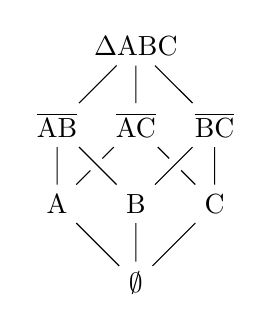
\begin{tikzpicture}
    \node (abc) at (0,2) {$\Delta$ABC};
    \node (ab) at (-1,1) {$\overline{\rm AB}$};
    \node (ac) at (0,1) {$\overline{\rm AC}$};
    \node (bc) at (1,1) {$\overline{\rm BC}$};
    \node (a) at (-1,0) {A};
    \node (b) at (0,0) {B};
    \node (c) at (1,0) {C};
    \node (o) at (0,-1) {$\emptyset$};
    \draw (o) -- (a) -- (ab) -- (abc) -- (ac) -- (c)
    (b) -- (o) -- (c) -- (bc) -- (abc)
    (a) -- (ac);
    \draw[preaction={draw=white, -,line width=6pt}] (ab) -- (b) -- (bc);
  \end{tikzpicture}
\end{center}

Each node of the Hasse diagram represents an element of $\Delta$ABC,
including both the whole triangle at the top
and the \textbf{null face} $\emptyset$ at the bottom.
\footnote{$\emptyset$, also known as the \textbf{nullitope}, is a convenient edge case.
  It has no vertices or other elements,
  and it is considered to be $-1$-dimensional!}
Whenever two nodes of the diagram are connected,
the higher node's element contains the lower element as a facet.
For example, the edge $\overline{\rm AC}$ contains the vertex C,
so their nodes are connected in the diagram with $\overline{\rm AC}$ above C.
Notice that the structure of the diagram does not depend on where the vertices are;
a scalene triangle would have the same Hasse diagram as the equilateral $\Delta$ABC.
A diagram considered on its own, without mention of the vertices' locations,
is also known as an \textbf{abstract polytope}.

Although every polytope can be represented by a Hasse diagram,
not every diagram represents a polytope.
For example, removing edge $\overline{\rm BC}$ from $\Delta$ABC
produces a new figure (left) and Hasse diagram (right):

\begin{center}
  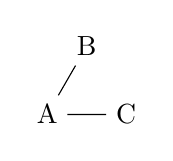
\begin{tikzpicture}
    \node (a) at (0,0) {A};
    \node (b) at (0.5,0.866) {B};
    \node (c) at (1,0) {C};
    \draw (c) -- (a) -- (b);
  \end{tikzpicture}
  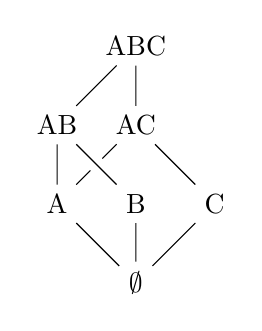
\begin{tikzpicture}
    \node (abc) at (0,2) {ABC};
    \node (ab) at (-1,1) {AB};
    \node (ac) at (0,1) {AC};
    \node (a) at (-1,0) {A};
    \node (b) at (0,0) {B};
    \node (c) at (1,0) {C};
    \node (o) at (0,-1) {$\emptyset$};
    \draw (o) -- (a) -- (ab) -- (abc) -- (ac) -- (c)
    (b) -- (o) -- (c)
    (a) -- (ac);
    \draw[preaction={draw=white, -,line width=6pt}] (ab) -- (b);
  \end{tikzpicture}
\end{center}

Note, however, that this requirement applies only to polygons.
To generalize it to $n$-polytopes,


\section{Regular polytopes}
There are multiple definitions for when a polytope is \textbf{regular},
but they all require every element (vertices, edges, faces, etc.) to ``look the same.''

\section{Uniform polytopes}
General polytopes can be very complicated. Therefore, we only tend to study specific categories of polytopes. The type of polytopes we study most in this server are \textbf{uniform polytopes}.

Uniformity is defined recursively. In 2D, uniform polytopes are simply the regular polygons.
In higher dimensions, uniform polytopes are those whose facets are all uniform. To see what we mean, let's look at a few examples.

\begin{figure}[H]
  \centering
  \begin{subfigure}{.33333\textwidth}
    \centering
    \includegraphics[width=.5\linewidth]{tut}
    \caption{Truncated tetrahedron}
    \label{fig:tut}
  \end{subfigure}%
  \begin{subfigure}{.33333\textwidth}
    \centering
    \includegraphics[width=.5\linewidth]{did}
    \caption{Dodecadodecahedron}
    \label{fig:did}
  \end{subfigure}%
  \begin{subfigure}{.33333\textwidth}
    \centering
    \includegraphics[width=.5\linewidth]{snid}
    \caption{Snub icosidodecahedron}
    \label{fig:snid}
  \end{subfigure}%
  \caption{Three examples of uniform polyhedra.}
  \label{fig:uniforms3D}
\end{figure}

In 3D, the uniform polytopes have already been enumerated. It turns out that, aside from the infinite families of \textbf{prisms} and \textbf{antiprisms}, there's exactly 75 uniform polyhedra.

\begin{figure}[H]
  \centering
  \begin{subfigure}{.5\textwidth}
    \centering
    \includegraphics[width=.5\linewidth]{hep}
    \caption{Heptagonal prism}
    \label{fig:hep}
  \end{subfigure}%
  \begin{subfigure}{.5\textwidth}
    \centering
    \includegraphics[width=.5\linewidth]{heap}
    \caption{Heptagonal antiprism}
    \label{fig:heap}
  \end{subfigure}%
  \caption{An example of a prism and an antiprism. These can be built from any regular polygon, and made uniform in all cases.}
  \label{fig:prisms}
\end{figure}

In 4D and higher up, the problem remains unsolved. In 4D, we know of two infinte families and 2194 uniform polychora. In 5D and up, we haven't yet done a thorough examination, though we know of various families of uniforms such as \textbf{Wythoffians} (those generated by a Coxeter diagram), and \textbf{multiprisms}.

\section{CRF polytopes}
A polytope is called \textbf{convex regular-faced}, or \textbf{CRF} for short, when it is convex (without dents, holes or self-intersections) and all of its faces are regular. Let's look at a few examples.

\begin{figure}[h]
  \centering
  \begin{subfigure}{.33333\textwidth}
    \centering
    \includegraphics[width=.5\linewidth]{Sphenomegacorona}
    \caption{Sphenomegacorona}
    \label{fig:polyhedra_1}
  \end{subfigure}%
  \begin{subfigure}{.33333\textwidth}
    \centering
    \includegraphics[width=.5\linewidth]{Hebesphenomegacorona}
    \caption{Hebesphenomegacorona}
    \label{fig:polyhedra_2}
  \end{subfigure}%
  \begin{subfigure}{.33333\textwidth}
    \centering
    \includegraphics[width=.5\linewidth]{Disphenocingulum}
    \caption{Disphenocingulum}
    \label{fig:polyhedra_3}
  \end{subfigure}%
  \caption{Test images!}
  \label{fig:polyhedra}
\end{figure}

\end{document}
